% Ausarbeitung SAJ 
% FH Augsburg 
%
%
%
%
\documentclass[titlepage, 12pt,a4paper]{scrartcl}
%scrartcl
\usepackage[ngerman]{babel}
%\usepackage[latin1]{inputenc}
\usepackage[T1]{fontenc}
\usepackage{ucs}            % Eventuell benötigt
\usepackage[utf8x]{inputenc}

\usepackage{setspace}           % Paket fuer den Zeilenabstand
\onehalfspacing                 % Setzt den Zeilenabstand auf 1.5

\usepackage{graphicx}
\usepackage{listings}
\usepackage[hyphens]{url}
%\usepackage{breakurl}
\usepackage{hyperref}
\usepackage[usenames]{color}
\definecolor{light-gray}{gray}{0.90}
\usepackage[fixlanguage]{babelbib}
\usepackage{listings}
%\lstset{numbers=left, numberstyle=\tiny, numbersep=5pt}
%\lstset{language=Perl}
\lstloadlanguages{bash,XML,HTML, PHP}
\selectbiblanguage{german}
\usepackage{makeidx}
%\usepackage{pifont}
\makeindex
%\usepackage{fancyhdr}
%\setlength{\headheight}{15.2pt}
%\pagestyle{fancy}


\author{Stephan Urban \& Andrés Cuartas}
\title{- Ausarbeitung - \\ Softwarearchitekturen in Java \\}
%\date{11-Dez-2007}

\pagestyle{myheadings}
\markright{Urban \& Cuartas}
\lstset{
	inputencoding=utf8x,
	extendedchars=\true,
	language=XML,
	basicstyle=\tiny,
	keywordstyle=\bfseries\color{green},
	identifierstyle=,
	%commentstyle=\color{gray},	
	%stringstyle=\itshape\color{darkred},
	numbers=left,
	numberstyle=\tiny,
	stepnumber=1,
	breaklines=true,
	frame=none,
	showstringspaces=false,
	tabsize=4,
	backgroundcolor=\color{light-gray},
	captionpos=b,
	float=htbp,
	frameround=fttt
}


%\lstset{language=XML, stringstyle=\ttfamily, tabsize=2, basicstyle=\small, breaklines=true, backgroundcolor=\color{light-gray}, frameround=fttt}
%              
% WORKAROUND, damit lstlistoflistings funktioniert: 
% Quelle: http://www.komascript.de/node/477
%
\makeatletter% --> De-TeX-FAQ
\renewcommand*{\lstlistoflistings}{%
  \begingroup
    \if@twocolumn
      \@restonecoltrue\onecolumn
    \else
      \@restonecolfalse
    \fi
    \lol@heading
    \setlength{\parskip}{\z@}%
    \setlength{\parindent}{\z@}%
    \setlength{\parfillskip}{\z@ \@plus 1fil}%
    \@starttoc{lol}%
    \if@restonecol\twocolumn\fi
  \endgroup
}
\makeatother% --> \makeatletter 

\begin{document} 

\maketitle

\newpage
\tableofcontents
\newpage

\section{Einführung}
Im Rahmen des Wahlpflichtfaches Softwarearchitekturen in Java haben wir die
Aufgabe unser Teilprojekt "Lehrevaluation", sowie den Spezialbereich 
„Java Server Faces“ in einer Ausarbeitung zu dokumentieren. 

Im Folgender Ausarbeitung werden wir auf die Teilbereiche bzw. Milesteones
eingehen. Einen überblick über den übertragenen Spezialbereich geben und
Probleme und Lösungen darstellen, auf die wir gestoßen sind. 

Die Abschnitte enden mit dem Zeichen des jeweiligen Autors. Wobei {\bf{AC}} für Andres
Cuartas und {\bf{SU}} für Stephan Urban verwendet wurde.
{\bf{AC}}
\section{Domain Modell}
Nachdem wir das Teilprojekt „Lehrevaluation“ zugelost bekamen, machten wir uns
erstmal Gedanken darüber wie während des Verlaufs unserer Studienzeit bisher
Lehrevaluationen durchgeführt wurden. Evaluationen verliefen alle auf ähnliche
Weise, dabei bekommen Studenten immer einen Fragebogen der im Normalfall so
aufgeteilt ist, dass Noten vergeben werden können. Ein Teilbereich für den
Gesamteindruck einer Vorlesung, ein anderer über Fachliche Aspekte und im
dritten Teil kann der Student Kommetare bzw. Verbesserungsvorschläge an dern
Professor richten. Natürlich verläuft die Evaluierung anonym und in Papierform
ab.

Unsere Aufgabe bestand darin diesen Verlauf zuerst durch Anforderungen in Form
von Userstories umzusetzen, um ein Gefühl dafür zu bekommen, was bei einer
Evaluierung auf der Seite der Studenten gefordert wird und auch was ein
Professor für Administrationsaufgaben hat, wenn er eine  Evalutaion erstellt.
Auch sollte ein Administrator berücksichtigt werden, der über alle nötigen
Rechte und die größte Übersicht auf Lehrevaluationen erhält. 

Mit Hilfe folgender Userstories haben wir die grundsätzlichen Anforderungen an
das System herausgearbeitet und uns einen Überblick verschafft.  

\begin{enumerate}
\item Student: 
\begin{enumerate} 
\item Auswahl verschiedener Fächer, abhängig vom Studiengang, bei denen entweder eine Evaluation möglich ist, bzw. diese abgeschlossen ist.
\item Anzeige der Evaluationsergebnisse
\item Student hat Evaluationsbogen vor sich und im ersten Abschnitt für Kriterien Noten vergeben
\item Im zweiten Abschnitt kann Lob/Kritik oder Anmerkungen schriftlich äußern
\item Am Ende wird eine Zusammenfassung angezeigt, die noch editierbar ist
\item Speichern/Übermitteln der Evaluation 
\end{enumerate}

\item Kriterien aus dem ersten Teil sind:

\begin{enumerate}
\item Niveau
\item Material
\item Vermittlung des Stoffs
\item Praxisbezug
\item Roter Faden
\item Eingehen auf Fragen
\item Arbeitsaufwand
\item Übungen
\item Gesamtbeurteilung der Veranstaltung 
\end{enumerate}

\item Professor: 
\begin{enumerate}
\item Beim Klick auf Evaluation starten, wird diese für alle Studenten
\item freigeschaltet. Beim Klick auf editieren werden, 
die Durchschnittswerte der einzelnen Noten angezeigt, sowie alle
schriftlichen Bewertungen. Die schriftlichen Bewertungen können auf dieser
Seite einzeln zur Veröffentlichung freigegeben bzw. wieder entfernt werden.

\end{enumerate}

\item Mitarbeiter: 
\begin{enumerate}
\item Kann im Grunde alles, was der Professor kann, im werden alle Evaluationen
aufgelistet.
\end{enumerate}

\end{enumerate}

In dieser Phase gab es insofern Probleme, dass wir eingrezen mussten wie
flexibel bzw. wie tief die einzelnen Personen das System betrachten dürfen. Es
musste also ein Mittelweg gefunden werden, welche fundamentalen funktionen das
System bieten sollte und was, um die Übersicht und die Umsetzung des
Teilgebiets so funktional und einfach wie möglich zu halten, weggelassen werden
sollte. Hierbei ist die Entscheidung gefallen den Mitarbeiter entfallen zu
lassen, weil dieser im Vergleich zum Professor nicht mehr Funktionalität inne
hat. 
{\bf{AC}}
\section{Klassenentwurf}
Um so effizient wie möglich am Projekt arbeiten zu könnnen, wurde überlegt, wie
die Zusammenarbeit durchgeführt werden sollte. Zu diesem Zeitpunkt hatten
wir die Möglichkeit GoogleWave einzusetzen. Zuvor war die Überlegung
Informationen im Projektwiki festzuhalten bzw. dort direkt zu bearbeiten. Die
Entscheidung fiel dann so, dass prototypisch unter GoogleWave Informationen
ausgetauscht wurden und wenn etwas dann für die Allgemeinheit festzuhalten war,
diese Informationen ins Wiki übeartragen wurde. 

\begin{figure}[h]
\begin{center}
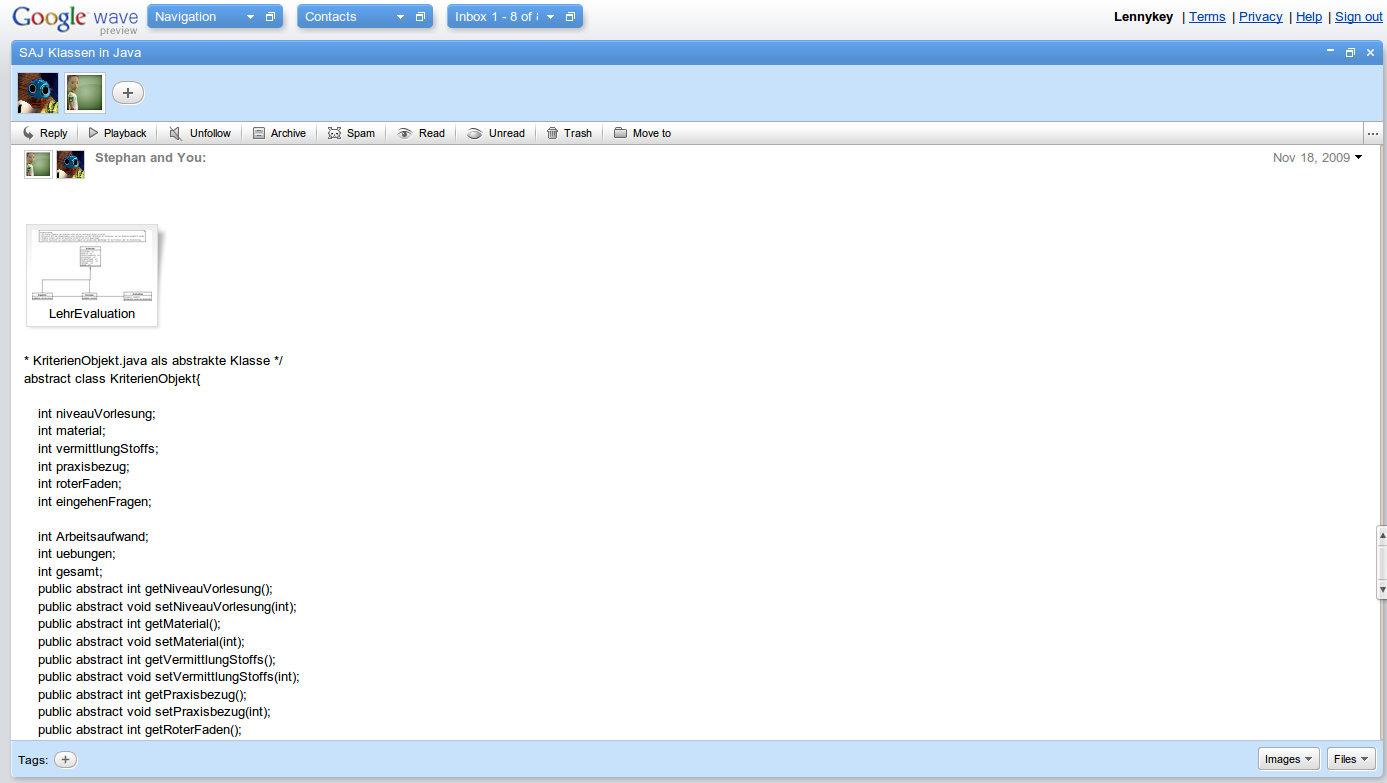
\includegraphics[width=15cm, height=12cm]{bilder/googleWave.png}
\caption{Google Wave}
\label{googleWave}
\end{center}
\end{figure}

So wurden Überlegungen des Klassenentwurfs unter GoogleWave diskutiert,
Teilergebnisse und fertige Klassendiagramme dann auf das Trac-Wiki
übertragen. Der Vorteil dieser Methode ist es, dass so die Gedanken und
Ideeenaustausch online und in echtzeit stattfinden konnte. So konnten Treffen
und die Fahrten in die FH entfallen und effizienter Zeit in das Projekt
einfließen.

So entstand ein Grobentwurf der Klassen zuerst in der Diskussion und mit Hilfe
von Opensource UML-Tools wie Umbrello, da unsere studentische Lizenzen für
VisualParadigm bereits abgelaufen waren. Leider lief Umbrello nicht so stabil,
so dass ein alternatives Tool gesucht wurde. Die Wahl fiel dann auf „DIA“, um
unsere Idee für das Klassendiagramm zu visualisieren, welches auf für
Netzwerkdiagramme benutzt werden kann. Da wir unter Java noch nicht so viel
Erfahrung mitbrachten erstellten wir dann aus dem Diagramm erstmal die Klassen
mit Hilfe von C++ Code, das aber ohne weiter Probleme später in Java-Code
umgeschrieben werden konnte.

\begin{figure}[h]
\begin{center}
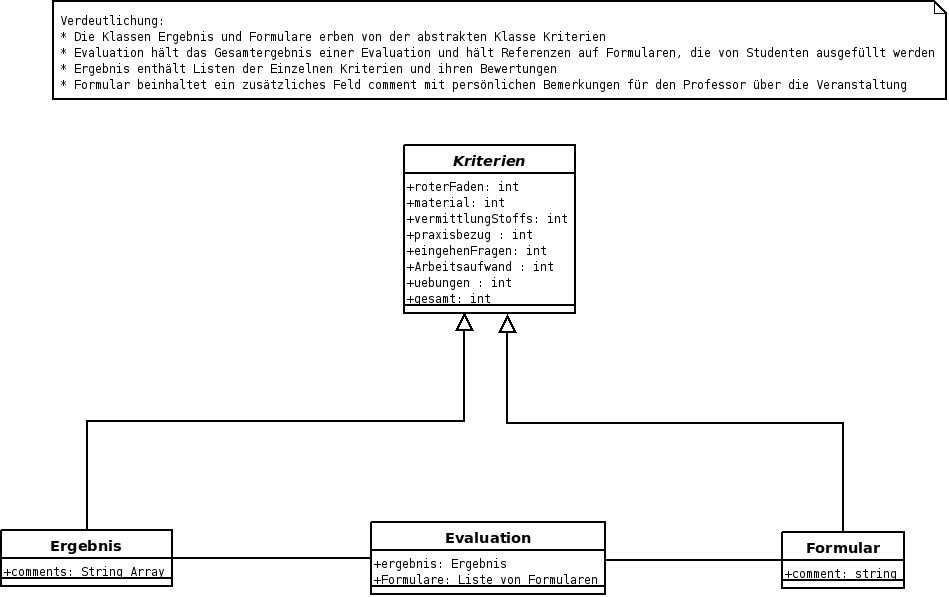
\includegraphics[width=15cm, height=12cm]{bilder/LehrEvaluation.png}
\caption{Klassenentwurf}
\label{Klassen}
\end{center}
\end{figure}

Die ersten Entwürfe wurden dabei mehrmals überarbeitet bis ein Klassendigramm
entstand, welches unsere Bedürnisse an das System einigermaßen gedeck hat.
Dabei ist uns erst nach Durchsicht von Prof. Meixner aufgefallen, dass
Kommentare der Studenten zu doppelt gespeichert wurden und zwar in einem
Formular selbst, wie auch in der Liste der Ergebnisse. Im
Klassendiagramm wurde auch noch nicht berücksichtigt, dass die Ergebnisse
Durchschnittswerte darstellen, die aber in der Parent-Class als Integer Werte
deklariert wurden. Es wurden weiterhin Redundanzen in den Setter und Getter
Methoden festegestellt und der Bezug einer Evaluierung zu einer
Lehrveranstaltung fehlte noch. Zu diesem Zeitpunkt waren die DAOs und die
Serviceschicht in Planung so dass das Weiterleiten der Ergebnisse an die
Serviceschicht und somit an die Weboberfläche noch nicht möglich war. 

Die obengenannten Punkte konnten dann ohne weitere Probleme behoben werden und
so konnten wir die Implementierung der DAOs und der Serviceschicht angehen. 
{\bf{AC}}
\section{Entwicklungsumgebung}
\subsection{Netbeans}
Ich habe über weite Teile des Projekts entgegen der Vereinbarung auf Netbeans
zurückgegriffen. Da es sich im begrenzten Umfang des Projekts leichter Bedienen
lies. Diese Entscheidung sollte sich bei der Entwicklung der Weboberfläche
noch als Vorteilhaft erweisen. Aber die Vorteile haben sich schon am Anfang gezeigt
da Eclipse die Projektstruktur nicht automatisch erkannte, sondern nur wenn man
das gesamte Projekt über das Subversion-Plugin ausgecheckt hatte. Netbeans hingegen
begnügt sich mit einer pom.xml. Somit war ich nicht an die IDE gebunden, sondern konnte
auch über Kommandozeile oder Tortoisse meine Sourcen verwalten.

\begin{figure}[htb]
\begin{center}
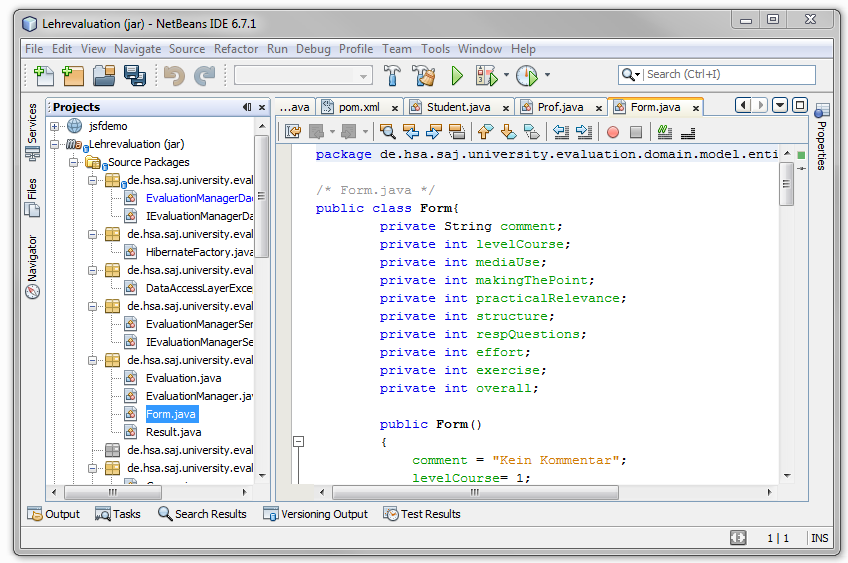
\includegraphics[width=12cm, height=7cm]{bilder/Netbeans.PNG}
\caption{Netbeans}
\label{netbeans}
\end{center}
\end{figure}

Die Arbeit mit Subversion war ich schon aus den Praktika gewohnt und konnte
somit meinem Teamkollegen beim Einstieg helfen.

Das Ticketsystem haben wir am Anfang noch beachtet aber im laufe des Semesters
immer weiter aus den Augen verloren. Die Kommunikation fand zum Ende hin vor allem
Gruppen intern statt.
{\bf{SU}}

\subsection{Eclipse}
Auf der anderen Seite habe ich mich für Eclipse entschieden, nachdem ich mit
Vim nicht mehr so effizient weitergekommen bin. Zwar hatte ich Netbeans
ausprobiert, wie mein Kommilitone, was auch sehr einfach zu bendienen ist, doch
fiel die Wahl, wegen der größeren Plugin Auswahl auf Eclipse. Auch Subversion
war auf der Kommandozeile unter Linux nicht mehr ganz so komfortabel. Es kostete
etwas Zeit bis mir der Umgang mit Eclipse leichter von der Hand fiel, vor allem
die Umgewöhnung von Vim auf das „normale“ editieren kostete Zeit. Das Editieren
gestaltete sich im späteren Verlauf etwas besser nach dem Installieren des
\emph{Vrapper}-Plugins, welches ermöglicht in Vim gewohnter Art, code zu
schreiben. Dabei legt sich das Plugin um verschiedene Eclipse-Editoren und ist
so unter Eclipse vielzeitig verwendbar, obwohl nicht das ganze Spektrum von
Eclipse angeboten wird. Ein weiterer Punkt war es sich für das richtige Eclipse
Paket zu entscheiden. Im Hinblick auf eine später Einbindung einer
Weboberfläche habe ich mich für die J2EE Variante in der Galileo Version
entschieden. Zwar wird man von Eclipse am Anfang von der Funktionalität
erschlagen und es mussten weitere Pakete nachinstalliert werden, wie z.B. für
die Arbeit mit dem Repository, aber der Umstieg auf Eclipse hat sich im Verlauf
des Projekts gelohnt. Vor allem deswegen, weil der Abgleich mit dem Repository
als effizienter und leichter erwies als auf der Konsole. Als weiter vorteilhaft
erwies sich dann auch das Einbinden eines Web-Projektes und die automatische
Generierung der Ordnerstruktur und der Konfigurationsdateien.


{\bf{AC}}


\section{Persistenz}
Um die Ergebnisse einer Evaluation zu sichern, wurde überlegt, was wirklich
persistent gehalten werden sollte, um Redundanzen so gering wie möglich zu
halten.

So ist es in unserem Teilprojekt nicht wichtig die Formulare mit samt den
Kommentaren einzeln zu speichern. Denn falls ein Formular bearbeitet wird,
werden die Durchschnittswerte in die Evaltuation verrechnet. Diese
Durchschnittswerte werden nach Beendigung der Evaluation nicht mehr verändert in
Folge werden nur dieser Ergebnisse persistent gehalten und nicht die enzelnen
Formulare. Auch die Kommentare zu der Evaluation werden in Verbindung zur
diesen gespeichert. Ein weiterer Vorteil ist, dass so, bei der Ausgabe,
die Ergebnisse nicht aus den einzelnen Formularen immer wieder neu berechnet
müssen sondern sofort zur Verfügung stehen und somit schneller zurückgegeben
werden können, z.B. an die Weboberfläche.

Ein Nachteil dabei ist, dass die Transparenz nicht mehr gewahrt bleibt, da die
Einzelergebnisse/Formulare nicht mehr existieren. Es sei denn die Formulare
werden in Papierform zur Verfügung gestellt und dann erst ins System
eingegeben, aber dieser Umweg soll durch dieses Teilprojekt vermieden werden
und jeder Student sollte die Möglichkeit bekommen online Formulare auszufüllen.


Aus diesen Überlegungen haben wir folgende Datenbank-Tabellen erarbeitet.

\begin{enumerate}
\item 08\_results:
\begin{enumerate}
\item CourseID(PK)
\item Result 
\end{enumerate}

\item 08\_students:
\begin{enumerate}
\item CourseID(PK)
\item StudID(PK)
\end{enumerate}
\end{enumerate}


Diese werden nun in die DAO mit Hibernate genutzt. Mit folgendem Codeausschnitt werden einfach
alle Studenten ausgelesen die bei einer Evaluation schon abgestimmt haben. Wobei „course“ ein long
und „students“ eine Liste von long ist.
\begin{lstlisting}[caption=Hibernate]{Hibernate}
	Query query = session.createQuery("select StudID from 08_students where courseid = " + course);
	students = query.list();
\end{lstlisting}

Da wir kein Spring verwendet haben mussten wir eine SessionFactory und eine Exception implementieren,
hierbei konnten wir uns dankenswerterweiße an die Implementierung von Gruppe 3 halten. Somit haben
wir vor jedem Query erst eine Session über die Factory angefragt und die Exceptions während dessen 
abgefangen. Wichtig war hierbei nicht zu vergessen Hibernate über die pom.xml einzubinden.
{\bf{SU}}
\section{Services}
Bevor die Weboberfläche arbeiten kann müssen von der Business-Logik Services zur
Verfügung gestellt werden. Desweiteren ist die Business-Logik dafür zuständig, dass
über die DAO die Peristenz gewehrleistet wird. Als erstes muss nun überlegt werden
was benötigt wird.

\begin{enumerate}
\item Weboberfläche:
\begin{enumerate}
\item Anzeige der Ergebnisse
\item Einreichen von ausgefüllten Formularen
\item Überprüfen ob eine Evaluation für ein bestimmtes Fach bereits existiert
\item Überpfüfen ob ein Student bereits abgestimmt hat
\end{enumerate}

\item DAO:
\begin{enumerate}
\item Intiales Laden aus der Datenbank
\item Einreichen von ausgefüllten Formularen
\end{enumerate}
\end{enumerate}


In unserer Ausarbeitung besitzt der Service ein EvalutionsManagerDao-Objekt
und ein EvaluationsManager-Objekt, welches wiederum im besitzt aller Evalutionen ist.
Somit kann der Service bei jeder externen Anfrage die Datenstände persistent halten.

\begin{figure}[h]
\begin{center}
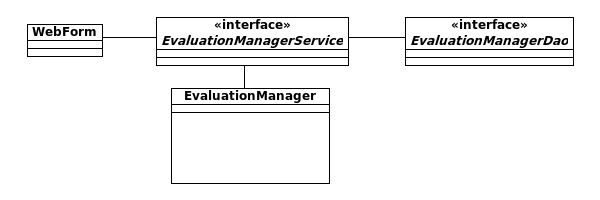
\includegraphics[width=15cm, height=5cm]{bilder/Service.png}
\caption{Service}
\label{service}
\end{center}
\end{figure}

Für die ausgearbeitete Problemstellung der Weboberfläche haben wir drei Funktionen erstellt.
Die einfachste hierbei ist die getResult()-Methode, da diese nur für eine gegebene courseID
ein Result-Objekt zurückliefert. Dieses wird hierfür von der courseID entsprechenden Evaluation
abgefragt.
Mit der login()-Methode lies sich sowohl die Problemstellung ob ein Student schon abgestimmt
hat als auch die ob eine Evaluation für ein bestimmtes Fach bereits existiert überprüfen. 
Diese Methode müsste auch immer vor dem betretten des Evaluationsbereichs aufgerufen werden.

Die letzte Methode für die Weboberfläche war die commitForm()-Methode. Dieser soll ein
ausgefülltes Formular übergeben werden, sowie die StudID und die courseID. Die Parameter
werden daraufhin an die commitForm()-Methode der Evaluation mit selbiger courseID übergeben.
Des daraus berechnete Ergebnis wird abgefragt und über den DAO auch gespeichert, ebenso der
Student anhand der StudID.

\begin{figure}[h]
\begin{center}
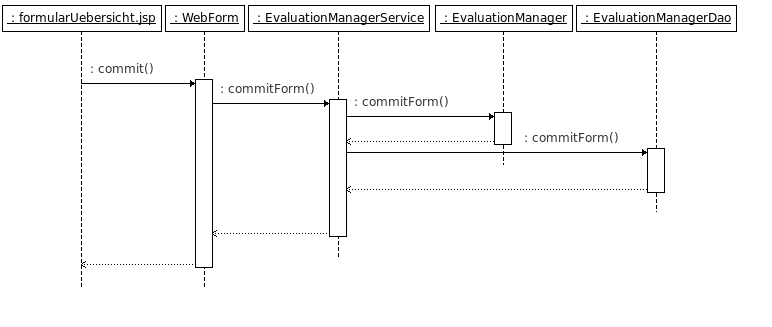
\includegraphics[width=15cm, height=5cm]{bilder/sequenceDiagram.png}
\caption{Sequenzdiagramm}
\label{sequenceDiagram}
\end{center}
\end{figure}

Bevor überhaupt etwas läuft müssen die Daten von vorherigen Sessions aus der Datenbank geladen werden.
Hierfür ist die initialize()-Methode zuständig. Diese lädt zuerst alle CourseIDs in eine Liste, 
dies geschiet mit der getAllCourses()-Methode von EvaluationManagerDAO. Daraufhin wird über die 
erstellte Liste iteriert und zu jedem Kurs die zugehörigen Results und Studenten-Listen geladen.
Aus den nun gewonnen Daten werden die zum jeweiligen Kurs gehörigen Evaluation mit addEvaluation()
zum EvaluationManager hinzugefügt.
{\bf{SU}}
\section{JUNIT Tests}
Da die Business-Logik bereits implementiert wurde, konnten auch schon die Unit-Tests
dazu erstellt werden. Hierfür haben wir JUnit verwendet. Es wurden fünf Test-Cases
erstellt. Davon einer zum Testen der commitForm()-Methode. Dabei wird für eine 
bereits in setUp() erstellte Evaluation ein Formular ausgefüllt und mit
commitForm() ins Result eingerechnet. Der Test besteht nun darin das durch
die Funktion abgespeicherte Result mit einem selbsterstellten Result mithilfe assertEquals zu vergleichen.

Die anderen vier Test-Cases beschäftigen sich mit der login()-Methode. Diesen sollen
alle vier Fälle beim Einsatz der login()-Methode abdecken. Nämlich erstens dass ein Professor die 
Evaluationsseite betritt, um sich die Ergebnisse anzuschauen. Hierfür muss die Evaluation schon
einmal erstellt worden sein. Deswegen benötigen wir die courseID die schon in der SetUp()-Methode
verwendet wurde. Wenn alles wie gewünscht funktioniert hat sollte, der zurückgegebene String "professor" lauten.
Der zweite Test-Case ist sehr ähnlich nur wird zusätzlich eine beliebige StudentenID übergeben. Dies funktioniert
weil die login()-Methode nur überprüft ob der jeweilige Student schon einmal teilgenommen hat.
Der dritte Test-Case erwartet nun einen Fehler-Code zurück. Den er übergibt eine CourseID, für die noch keine
Evalution erstellt wurde. Der letzte Test-Case bedarf ein wenig Vorarbeit. Hierfür wird das in der SetUp()-Methode
erstellte Formular mit der commitForm()-Methode zur Evaluation hinzugefügt. Somit hat der jeweilige Student schon
einmal abgestimmt, und es wird daher auch ein Fehler erwartet.

Auch wenn es nicht so viele Test-Cases sind, haben wir aber die Methoden gewählt die auch schon in der Web-Anwendung
benutzt werden. Auch werden alle Fehlerfälle abgedeckt.

In unseren ersten Ansätzen für die Tests haben wir das Prinzip der Test-Cases missverstanden. Da wir gegen das
Gebot der Isolation verstoßen haben, denn ein Unittest soll nur immer ein Modul alleine testen.
{\bf{SU}}

\section{Weboberfläche}
Mit Hilfe von JavaServerFaces ist es leicht möglich auf die die Methoden und
Attribute der Serviceschicht zuzugreifen. Deswegen haben wir uns dafür
entschieden für die Weboberfläche JSF einzusetzen. Auch aus den Guten
Erfahrungen während der Recherche zu unserem Spezialthema für die Vorlesung. 

Es gab leider beim Einsatz von CSS Probleme, um z.B. die Formulare zu
gestalten. Dabei ist es normalerweise so, dass man ein Stylesheet
folgendermaßen in HTML einbindet:

\begin{lstlisting}
<link rel="stylesheet" type="text/css" href="css/main.css">
\end{lstlisting}

Dabei wurde aber das Stylesheet unter „WebContent/css/main.css“ nicht gefunden,
bzw. wurden die Anweisungen ignoriert. Nach langer
Recherche\footnote{http://confluence.sakaiproject.org/display/BOOT/JSF+Adding+CSS} in verschiedenen JSF Foren konnten wir dann mit Hilfe von:

\begin{lstlisting}
<style type="text/css">
			@import url("css/main.css");
</style>
\end{lstlisting}

schließlich doch noch CSS-Definitionen erstellen und sie auf die Formulare
anwenden. Eine Erklärung, warum das standardmäßige Einbinden konnte leider
nicht gefunden werden.
Darüber hinaus kann man ohne Probleme DIV-Tags nutzen, um die Struktur der
einzelnen Seiten aufzubauen und so den Aufbau vom Design der Seite trennen. 

Hier eine Auswahl der mit Hilfe von JSF und CSS gestalteten Seiten:

\begin{figure}[h]
\begin{center}
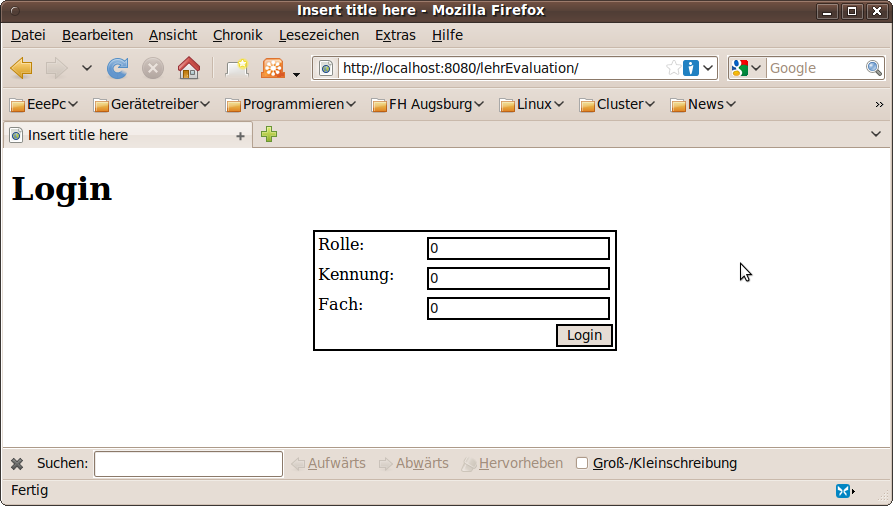
\includegraphics[width=15cm, height=10cm]{bilder/loginSeite.png}
\caption{Login}
\label{login}
\end{center}
\end{figure}

\begin{figure}[h]
\begin{center}
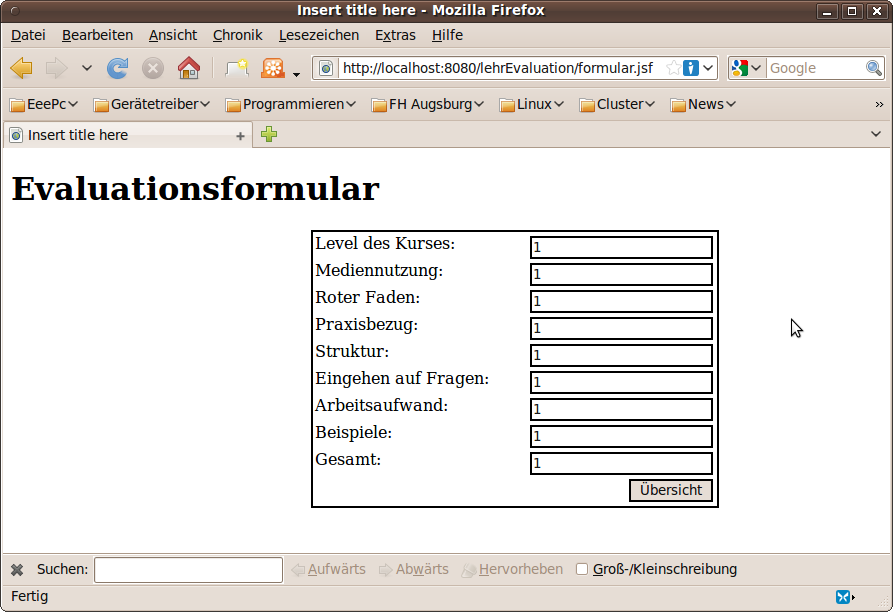
\includegraphics[width=15cm, height=10cm]{bilder/formular.png}
\caption{Formular}
\label{formular}
\end{center}
\end{figure}


Zuerst gelangt man, wenn man die Weboberfläche aufruft auf eine Login Seite,
bei der man abhängig der eingegebenen Parameter entweder auf eine Seite für
Studenten gelangt oder auf eine Seite, die nur für Professoren bestimmt ist.
Auf der Studentenseite ist es dann möglich ein Formular für ein Fach
auszufüllen. Das Fach ist ebenfalls abhängig, welches Fach vorher im
Login-Bereich ausgewählt wurde. Die andere Option auf der Studentenseite ist,
das Zwischen- bzw. Endergebnis der jeweiligen Evaluation einzusehen. Dem
Professor wird auf seiner Startseite nur gestattet die Ergebnisse zu einer von
ihm vorher ausgewälten Evaluation einzusehen. 

Die Weiterleitung auf die jeweils spezialisierten Seiten, also die für
Studenten oder für Professoren wird ermöglicht, durch die „faces-config.xml“
und der entsprechenden JavaBean, in diesem Fall die „WebForm.java“. Nach einem
Klick auf den Login Button wird abhängig von der Matrikelnummer ein
entsprechender Rückgabewert an die JSF-Longin Seite zurückgegeben. Die
entsprechende Weiterleitung wird in der faces-config.xml folgendermaßen
eingestellt: 

\begin{lstlisting}
<navigation-rule>
<from-view-id>/login.jsp</from-view-id>
<navigation-case>
<from-outcome>student</from-outcome>
<to-view-id>/student.jsp</to-view-id>
</navigation-case>
</navigation-rule>

<navigation-rule>
<from-view-id>/login.jsp</from-view-id>
<navigation-case>
<from-outcome>professor</from-outcome>
<to-view-id>/professor.jsp</to-view-id>
</navigation-case>
</navigation-rule>
\end{lstlisting}

Hier wird angegeben, was passieren soll, wenn auf der Seite „login.jsp“ ein
Button oder entsprechender Link geklickt wird und entweder „student“ oder
„professor“ zurückgegeben wird.

Ein entsprechender Button oder Link muss folgendermaßen in der Seiten
eingebunden werden:

\begin{lstlisting}
<h:form>
<h:commandButton action="#{webform.login}" value="Login" styleClass="floatRight" />
</h:form>
\end{lstlisting}

Wobei der entsprechende Button bzw. Link auf der Seite in einem JSF
\emph{<h:form>}-Tag eingebunden werden muss, um ausgewertet zu werden. Mit Hilfe der Expression-Language (EL) \emph{\#\{webform.login\}} werden die
enstsprechenden JavaBeans angestoßen. 
{\bf{AC}}
\section{Java Server Faces}
Am Anfang der Einarbeitung war es schwierig die vorhandenen Beispiele aus
Büchern bzw. dem Internet zum Laufen zu kriegen, auch deswegen, da es an
Erfahrung mit Eclipse fehlte. Im laufe des „Try and Error“ die richtige
Konfiguration unter Eclipse einzustellen, konnte letztendlich eine
Beispielanwendung zum Laufen gebracht werden. Dabei gibt es zwei verschiedene
Ansätze. 

Erster Ansatz, man bindet unter Eclipse z.B. den Tomcat Webserver ein und legt
alle benötigten Bibliotheken in den „WEB-INF/lib“ Ordner. Folgende Dateien
sollten für ein funktionierendes Java Server Faces Projekt eingebunden
bzw. kopiert werden. Die
JSTL\footnote{http://download.java.net/maven/1/jstl/jars/jstl-1.2.jar} Implementation, leider funktioniert die neuste Implementation, die man z.B. aus
dem Mojarra\footnote{https://jstl.dev.java.net/download.html} Projekt
runterladen nicht, weil ein paar Libraries fehlen ohne die man nicht auf Java
Server Pages zurückgreifen kann, um mit diesen zu arbeien. Darüberhinaus ist es
noch nötig, sich für eine JSF Implementation zu entscheiden. Für den Anfang
reicht es auf die Mojarra Implementation zurückzugreifen. Benötigt man weitere
Funktionalität bzw. weitere JSF-Tags die mehr Funktionalität bieten, lohnt es
sich mit Apache MyFaces auseinander zu setzen. 

Der andere Ansatz ist, die benötigten Bibliotheken als UserLibraries unter
Eiclipse einzubinden und diese dann in den Java Build Path mit aufzunehmen.
Darüberhinaus sollte auch beachtet werden, unter „Properties->Java EE
Module Dependencies“ die benötigten Bibliotheken zur Laufzeit einzubinden.



\begin{figure}[h]
\begin{center}
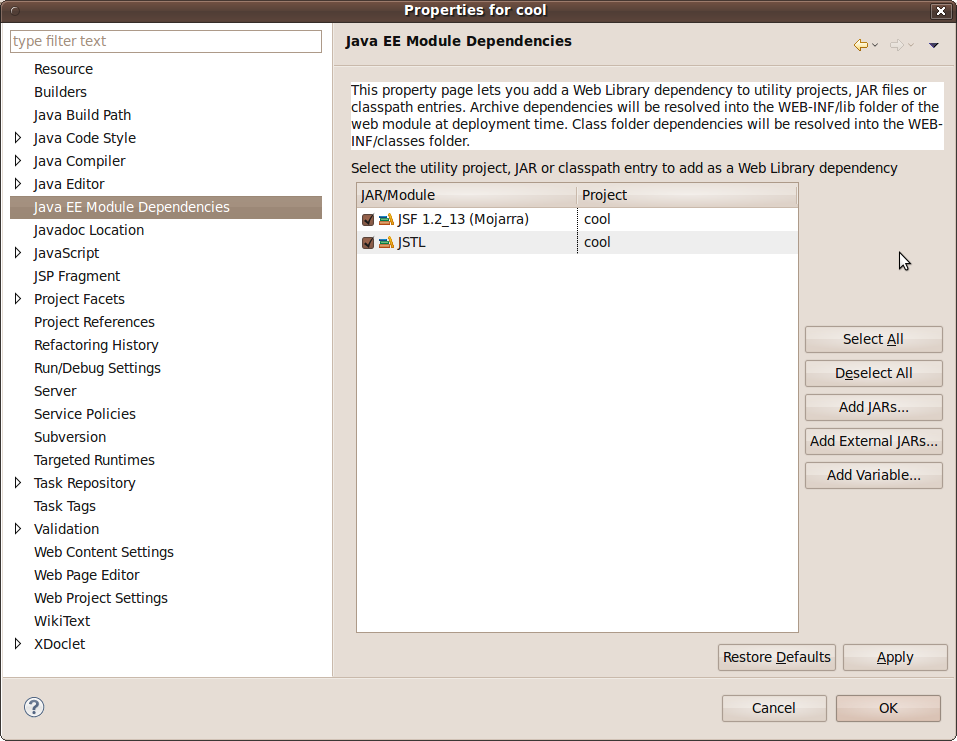
\includegraphics[width=15cm, height=10cm]{bilder/Properties.png}
\caption{Properties}
\label{properties}
\end{center}
\end{figure}

Wenn dieser Schritt ausgelassen wird, was im Laufe der Konfiguration
und mangels Erfahrung mit Eclipse oft passiert ist, kann der Webserver nicht
auf die benötigten Bibliotheken zugreifen und somit das Projekt nicht
ausführen.

Folgende Fehlermeldungen können dann in der Fehlerkonsole unter Eclipse
angezeigt werden:


\begin{verbatim}
SCHWERWIEGEND: Error configuring application listener of class
com.sun.faces.config.ConfigureListener
java.lang.ClassNotFoundException: com.sun.faces.config.ConfigureListener

org.apache.catalina.core.StandardContext listenerStart
SCHWERWIEGEND: Skipped installing application listeners due to previous
error(s)

org.apache.catalina.core.StandardContext start
SCHWERWIEGEND: Error listenerStart

\end{verbatim}

Wobei die angegebenen Java Klassen nicht gefunden werden, die sich z.B. in den
JSF Implementierungen oder in der JSTL befinden. 
{\bf{AC}}

Unter Netbeans gestaltet sich die Arbeit mit JSF um einiges einfacher. 
Zum einen werden die Bibliotheken automatisch eingebunden. Zum anderen
steht mit Visual JSF eine einsteigerfreundliche Alternative zur eigenhändigen
Erstellung der JSP-Seiten zur Verfügung. Denn Visual JSF bietet einen Designer
mit dem man die JSP-Seiten zusammenklicken kann, wobei jederzeit auch in den 
Editor gewechselt werden kann. Auch kann man mit diesem Designer die Verbindungen
zwischen JSP-Seiten und Java-Bean verwalten. Desweiteren bietet Visual JSF eine
große Auswahl an Objekten die, auch in der Java-Bean angesprochen werden können.
Letztenendes haben wir uns aber gegen Visual JSF entschieden da die angebotenen
Objekte nicht kompatibel mit Eclipse sind und sich unser Projekt auch mit
einfachen Elementen erstellen lassen kann.

\begin{figure}[htb]
\begin{center}
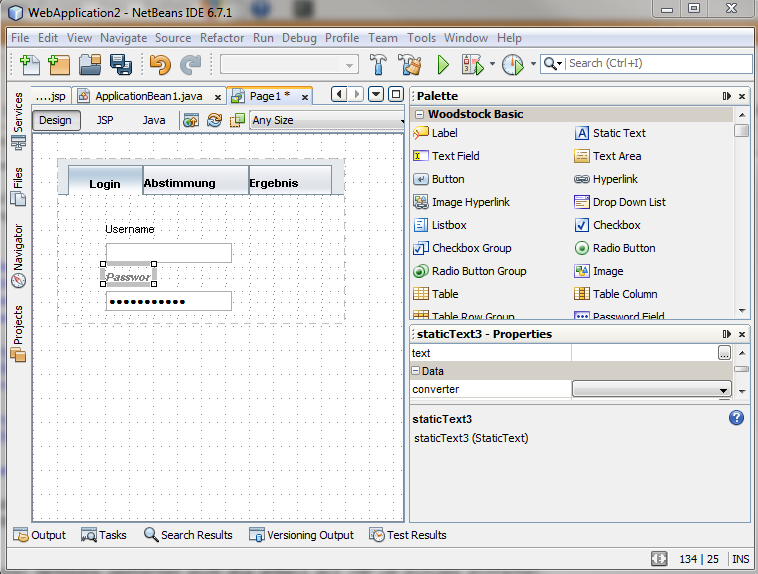
\includegraphics[width=15cm, height=10cm]{bilder/VisualJSF.png}
\caption{Visual JSF Designer}
\label{visual-jsf-designer}
\end{center}
\end{figure}

Desweiteren haben wir für den Vortrag und unserer Beratertätigkeit auch noch eine
weiteres Framework untersucht. Nämlich ICEfaces, dieses basiert auf AJAX und bietet
daher eine GUI-ähnliche Reaktionszeit. Auch werden schon einige Klassen und Tags zur 
verfügung gestellt.
Daher haben wir allgemein für Anfänger eine Empfehlung für Visual JSF und für ehrgeizigere
Projekte ICEfaces ausgesprochen. Für die Arbeit an dem Projekt sind die Refrenzimplementierung
Mojarra oder das ein wenig erweiterte Apache MyFaces vollkommen ausreichend. In unserer Demo
(jsfDemo.war siehe auf beigelegter CD) haben wir die für das Projekt wichtigsten Elemente
vorgeführt. Also Ein- und Ausgabefelder, sowie dazugehörige Validatoren und natürlich Buttons.
{\bf{SU}}
\section{Was noch Fehlt}
Durch die wenige Zeit konnten nicht alle Themengebiete in unserem Code abgedeckt werden. 
Auch ist durch die fehlende Parktikumsstunde keine richtige Kommunikation zustande gekommen.
Dieser Abschnitt soll nun die Aspekte aufzeigen die wir zwar durchdacht oder sogar geplant, aber
nicht implementiert haben. 
{\bf{SU}}

\subsection{Verbindung zu anderen Teilprojekten}
Durch die fehlenden Verbindungen zu den anderen Teilprojekten, haben wir zum einen noch Dummies im Einsatz,
zum anderen eine nicht so schöne Startseite, die einem zum Login auffordert. Diese Login-Funktionalität
hätte dann von der vorherigen Seite übernohmen werden können. 
\begin{figure}[htb]
\begin{center}
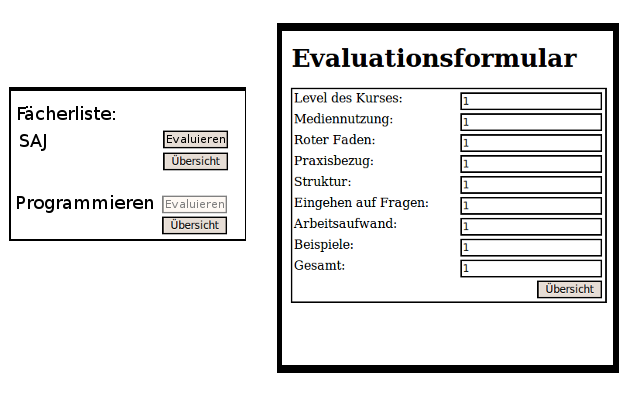
\includegraphics[width=15cm, height=10cm]{bilder/Connection.png}
\caption{Verbindung zwischen Fächerübersicht und Evaluationen}
\label{connection}
\end{center}
\end{figure}
Eine Idee wäre, dass das Veranstaltungsteam auf der Seite, wo ihre Veranstaltungen aufgelistet werden, für jede
Veranstaltung einen Button setzten (siehe Abbildung), oder eben auf der Profilseite der Veranstaltung. Auch könnte
der Button ausgegraut sein wenn momentan keine Evaluation möglich ist. Bei einem Klick auf den Button könnten die 
dahinter liegende Bean die Informationen des Benutzers und des jeweiligen Kurses an uns weitergeben. Die dafür
nötige Funktion stellt schon der EvaluationManagerSerivce zur Verfügung.{\bf{SU}}
\subsection{Sicherheit}
Durch die fehlende Verbindung zwischen den Projekten ist eine sache ganz deutlich unter den Tisch gefallen,
die Sicherheit. Zum einen findet bei uns keine richtige Authentifizierung statt, sondern wir nehmen diese
als gegeben an. Auch hätten wir um die Anonymität der Evaluation zu waren, eine Verschlüsselung ins Auge
fassen können.
{\bf{SU}}

Eine weitere Frage wäre, in wie fern wir unsere Eingabeformulare hätten noch schützen müssen.
Da in der Eingabezeile für den Kommentar auch folgendes hätte eingeben werden können:
\begin{lstlisting}
	test'); DROP TABLE Students;--
\end{lstlisting}
Was Hibernate in unserer jetztigen Implementierung wahrscheinlich ausgeführt hätte.
\subsection{Spring}
Vorallem bei der Implementierung von Hibernate hätte uns Spring einige Arbeit abnehmen können. Wenn man
sich unseren DAO-Code anschaut, wimmelt es da von try/catch-Blöcken. Diese hätte man sich mit Hibernate
einsparen können. Auch hätte sich das Session-Handling um einiges vereinfacht, da sich auch hier 
viel Boiler-Plate-Code hätte einsparen lassen.
{\bf{SU}}

Wir haben, wie aus dem Code ergeht, versucht eine rudimentäre
Sicherheitsschranke mit der Login-Seite einzubauen. Nach näherer Befassung mit
Spring hätten wir das wahrscheinlich mit Hilfe von Acegi leichter bzw.
flexibler lösen können. Auch eine Einbindung von JSF wäre mit Hilfe von Spring
wäre möglich gewesen, um unsere Beans mit Spring-Beans zu verbinden, um die
Kontrolle an Spring zu übergeben.{\bf{AC}}

\subsection{Mocking}
Bei den Unit-Test hätten wir noch Mocking einsetzten können um Fehler mit der Datenbank zu simmulieren.
{\bf{SU}}
\section{Credo}
\subsection{Andres Cuartas}
Vor der Vorlesung hatte ich nur vor dem Studium Kontakt mit Java. Mir sind die
Konzepte von Java zwar vertraut, aber die Praxis fehlte mir. Auch die
Einarbeitung in den verschiedenen Frameworks kostete viel Zeit, vor allem die
vielen kleinen Probleme mit JSF, um eine Testumgebung zum laufen zu bringen
kostete sehr viel Geduld. Auch deswegen, weil der neue Umgang mit Eclipse
nebenher laufen musste. 

Aus der Vorlesung nehme ich viel Praxiserfahrung mit und einen groben Umgang
mit den verschiedenen Frameworks. Leider bedauere ich im Nachhinein, dass wir
nicht gleich auf Spring gesetzt haben, was vieles hätte erleichtern können. 
{\bf{AC}}
\subsection{Stephan Urban}
Ich hatte vor der Veranstaltung sehr wenige Java-Kenntnisse, dafür aber mit C++ viel Erfahrung mit Objektorientierung
und Modularisierung. Aus der Veranstaltung nehme ich jedenfalls ein bischen fundiertere Kenntnisse in Java, ein guten
Überblick über eingesetzte Frameworks und Technicken, sowie einen tieferen Einblick in JSF mit. Wobei für mich das JSF
und die Patterns den größten praktischen Nutzen für mich haben.
{\bf{SU}}

\newpage % Ende des eigentlichen Inhalts

\listoffigures
%\lstlistoflistings
\printindex
\begin{thebibliography}{99}
\bibitem{}
Eberhard Woff: Spring 2, 2007 dpunkt.Verlag
\bibitem{}
Hans Bergsten: JavaServerFaces, 2004 O'Reilly
\bibitem{}
Sven Haiges: JavaServerFaces, 2006 Entwickler Press
\bibitem{}
Richard Oates: Spring und Hibernate, 2007 Carl Hanser Verlag
\bibitem{}
http://openbook.galileocomputing.de/javainsel8/
\bibitem{}
http://www.icefaces.org/main/ajax-java/jsf-components.iface
\bibitem{}
http://www.roseindia.net/jsf/validator.shtml
\bibitem{}
JSF-Linksammlung: http://www.clusterurl.com/496nn5l

\end{thebibliography}


\end{document}
